\documentclass[xcolor=x11names,compress,professionalfonts, aspectratio=169]{beamer}

%% General packages %%%%%%%%%%%%%%%%%%%%%%%%%%%%%%%%%%
\usepackage[utf8]{inputenc}
\usepackage{graphicx}
\usepackage{tikz}
\tikzset{% change default arrow tips
    >=latex
}
\usepackage{ifthen}

\usepackage{amsmath}
\usepackage{nicefrac}

\usepackage{color}

% compile child documents using this preamble
\usepackage{subfiles}

% compile child files with separate preambles, and include them in the document
\usepackage{standalone}

%%%%%%%%%%%%%%%%%%%%%%%%%%%%%%%%%%%%%%%%%%%%%%%%%%%%%%

\makeatletter
\setbeamertemplate{footline}
{
    \leavevmode%
    \hbox{%
        \begin{beamercolorbox}[wd=.333333\paperwidth,ht=2.25ex,dp=1ex,center]{author in head/foot}%
            \usebeamerfont{author in head/foot}\insertshortauthor
        \end{beamercolorbox}%
                \begin{beamercolorbox}[wd=.333333\paperwidth,ht=2.25ex,dp=1ex,center]{title in head/foot}%
            \usebeamerfont{title in head/foot}\insertshorttitle
        \end{beamercolorbox}%
        \begin{beamercolorbox}[wd=.333333\paperwidth,ht=2.25ex,dp=1ex,right]{date in head/foot}%
            \usebeamerfont{date in head/foot}\insertshortdate{}\hspace*{2em}
            \insertframenumber{} / \inserttotalframenumber\hspace*{2ex} 
        \end{beamercolorbox}}%
        \vskip0pt%
    }
    \makeatother


%% Beamer Layout %%%%%%%%%%%%%%%%%%%%%%%%%%%%%%%%%%
\useoutertheme[subsection=false,shadow]{miniframes}
\useinnertheme{rectangles}

\setbeamertemplate{navigation symbols}{}%remove navigation symbols

\author{Nicolas Macé}

\newcommand{\btVFill}{\vskip0pt plus 1filll}%place an element at the bottom of the page

\usepackage{libertine}
\usepackage[T1]{fontenc}

\setbeamerfont{title like}{shape=\scshape}
\setbeamerfont{frametitle}{shape=\scshape}

\setbeamercolor*{lower separation line head}{bg=DeepSkyBlue4} 
\setbeamercolor*{normal text}{fg=black,bg=white} 
\setbeamercolor*{alerted text}{fg=red} 
\setbeamercolor*{example text}{fg=black} 
\setbeamercolor*{structure}{fg=black} 
 
\setbeamercolor*{palette tertiary}{fg=black,bg=black!10} 
\setbeamercolor*{palette quaternary}{fg=black,bg=black!10} 

\renewcommand{\(}{\begin{columns}}
\renewcommand{\)}{\end{columns}}
\newcommand{\<}[1]{\begin{column}{#1}}
\renewcommand{\>}{\end{column}}

\definecolor{BostonBlue}{HTML}{00688B}
\definecolor{Complementary}{HTML}{8B2300}

% letters A and B appearing in the qp chains
\newcommand{\A}{\textcolor{BostonBlue}{A}}
\newcommand{\B}{\textcolor{Complementary}{B}}

\renewcommand{\ss}[1]{\scriptsize{\text{#1}}}
%%%%%%%%%%%%%%%%%%%%%%%%%%%%%%%%%%%%%%%%%%%%%%%%%%

\usepackage{braket}
% compile child documents using this preamble
\usepackage{subfiles}

%%%My Math

\newcommand{\pd}[2]{\frac{\displaystyle \partial #1}{\displaystyle\partial #2}} % for partial derivatives
\renewcommand{\d}[1]{\mathrm{d}#1}

\begin{document}

\begin{frame}
\title{{\fontsize{14}{60}\selectfont Exact results on electronic wavefunctions of 2D quasicrystals}}

\author{{\fontsize{10}{60}\selectfont Nicolas Macé$^1$, Anuradha Jagannathan$^1$, Pavel Kalugin$^1$, Rémy Mosseri$^2$, Frédéric Piéchon$^1$}}

\institute % (optional)
{
  $^1$Laboratoire de Physique des Solides, \emph{Université Paris-Saclay} \\
  $^2$LPTMC, \emph{Université Pierre et Marie Curie}
}

\date{June 20, 2017}

\titlepage

\btVFill
\begin{columns}
\begin{column}{2cm}
~\\
~\\
~\\
~\\
\raggedright

\includegraphics[scale=.15]{img/0_cover/LogoUPSUD.png}
\end{column}
\begin{column}{6cm}
\centering
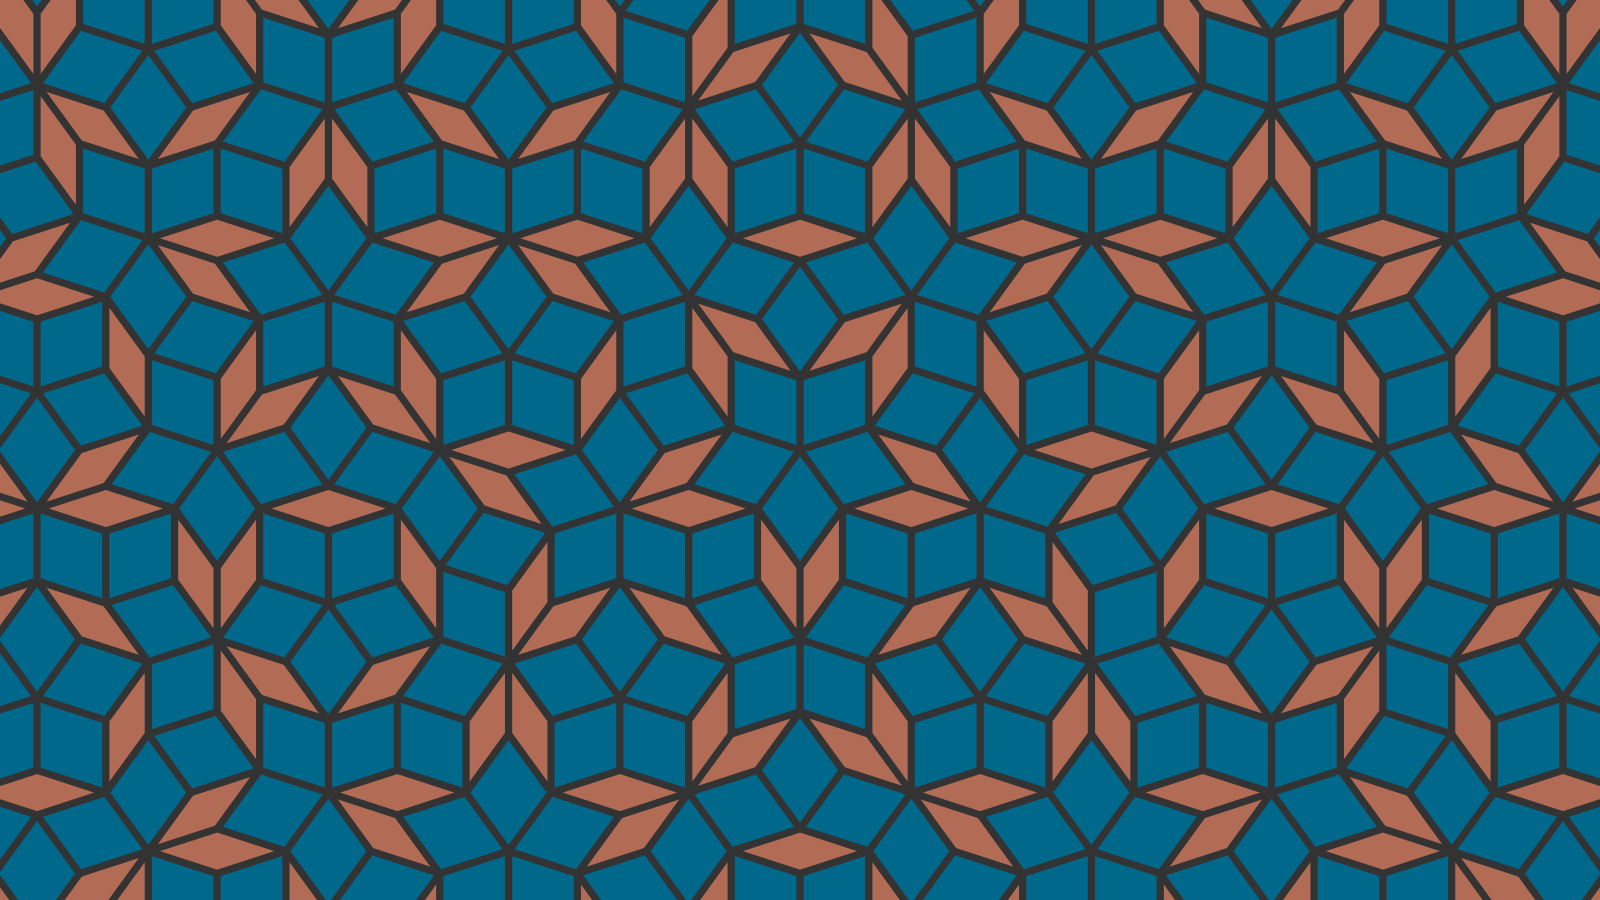
\includegraphics[width=.8\textwidth]{img/0_cover/cover.png}
\end{column}
\begin{column}{2cm}
~\\
~\\
~\\
~\\
\raggedleft

\includegraphics[scale=.15]{img/0_cover/logo-lps.jpg}
\end{column}
\end{columns}
\end{frame}

\section{La structure des quasicristaux}
%Each section needs a subsection for the small points on top to show up
\subsection{Dummy}
\begin{frame}{Quasicrystals}
Aperiodic yet ``ordered'' arrangement of atoms/molecules/colloids

A quasicrystal has the following properties:
\begin{itemize}
	\item it is \textbf{aperiodic}
	\item it is \textbf{long range ordered} (its diffraction pattern exhibits sharp peaks).
\end{itemize}
%\textbf{Aperiodic tilings} are used to model quasicrystals.
\(
	\<{6cm}
		\centering
		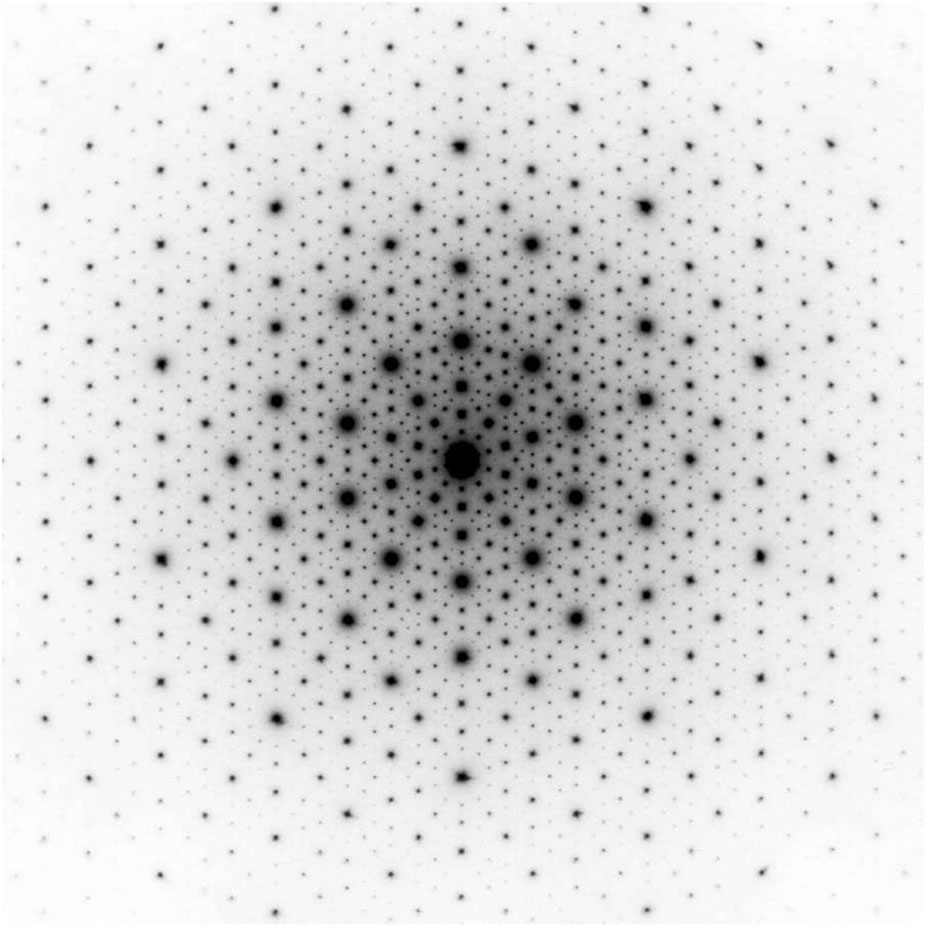
\includegraphics[scale=0.1]{img/1_intro/diffraction_tenfold.png}
		
		\ss{Figure de diffraction d'un alliage d'AlPdMn} \ss{(groupe de Conradin Beeli)}
	\>
	\<{6cm}
		\centering
		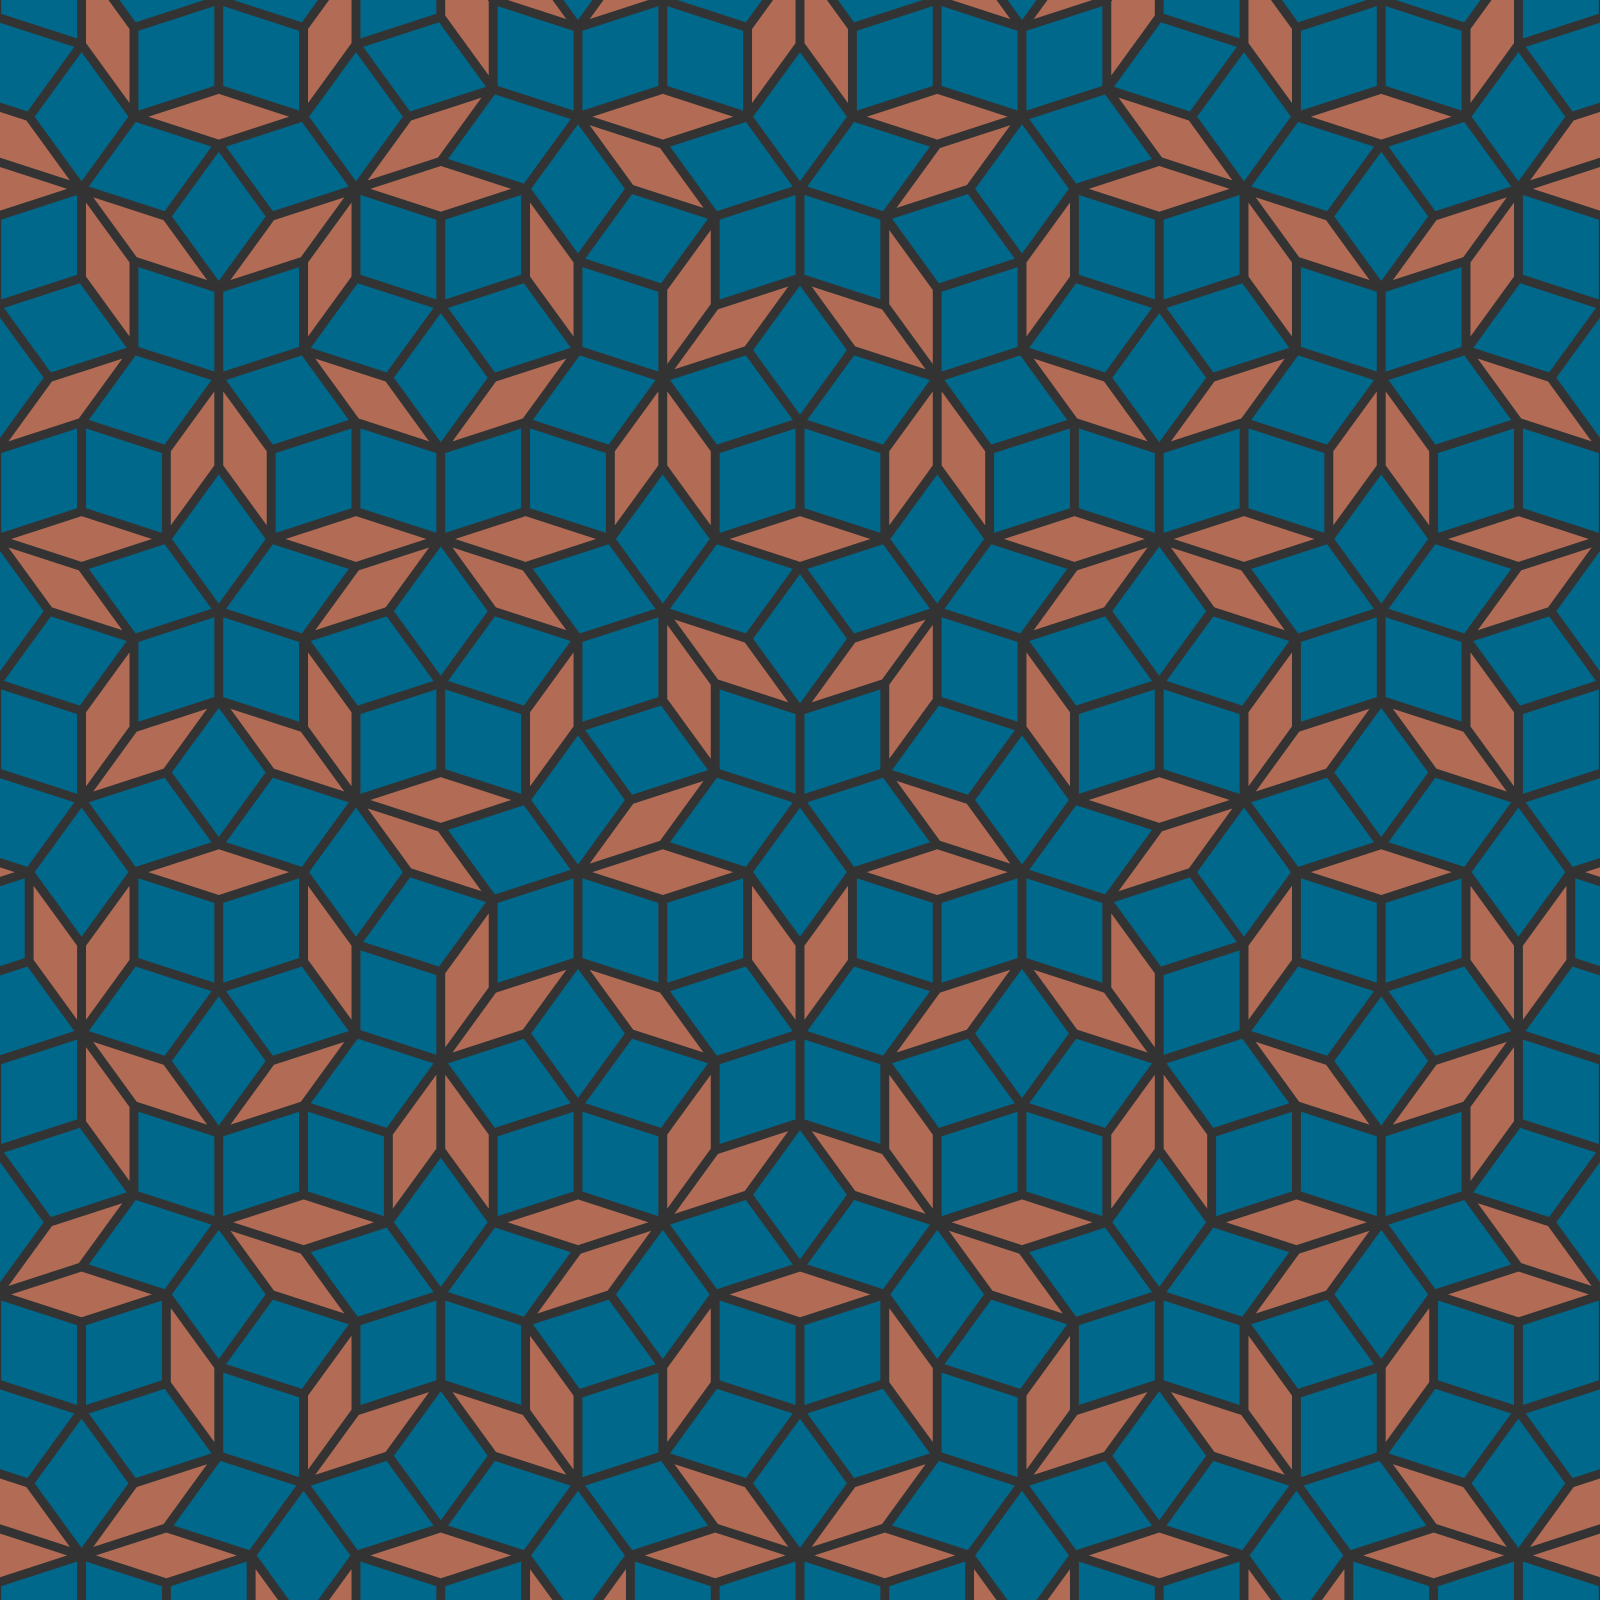
\includegraphics[scale=0.06]{img/1_intro/penrose.png}
		
		\ss{Un morceau du pavage de Penrose,} \ss{souvent utilisé pour modéliser les quasis.}
	\>
\)
\end{frame}

\begin{frame}{Exemples de quasicristaux}
\(
	\<{6cm}
		\centering
		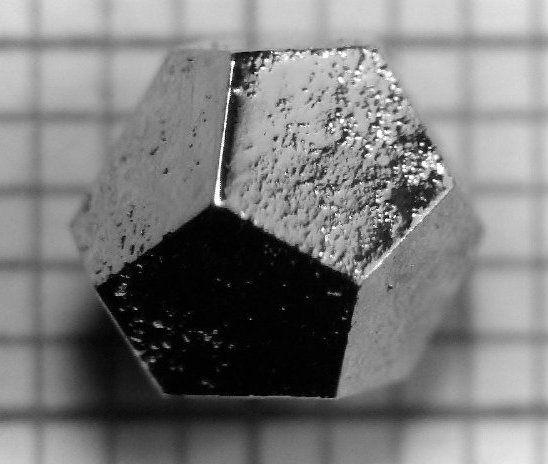
\includegraphics[scale=0.28]{img/1_intro/homgzn.png}
		
		\ss{HoMgZn alloy in its icosahedral phase} \ss{(\url{doi:10.1038/nmat1244})}
	\>
	\<{6cm}
		\centering
		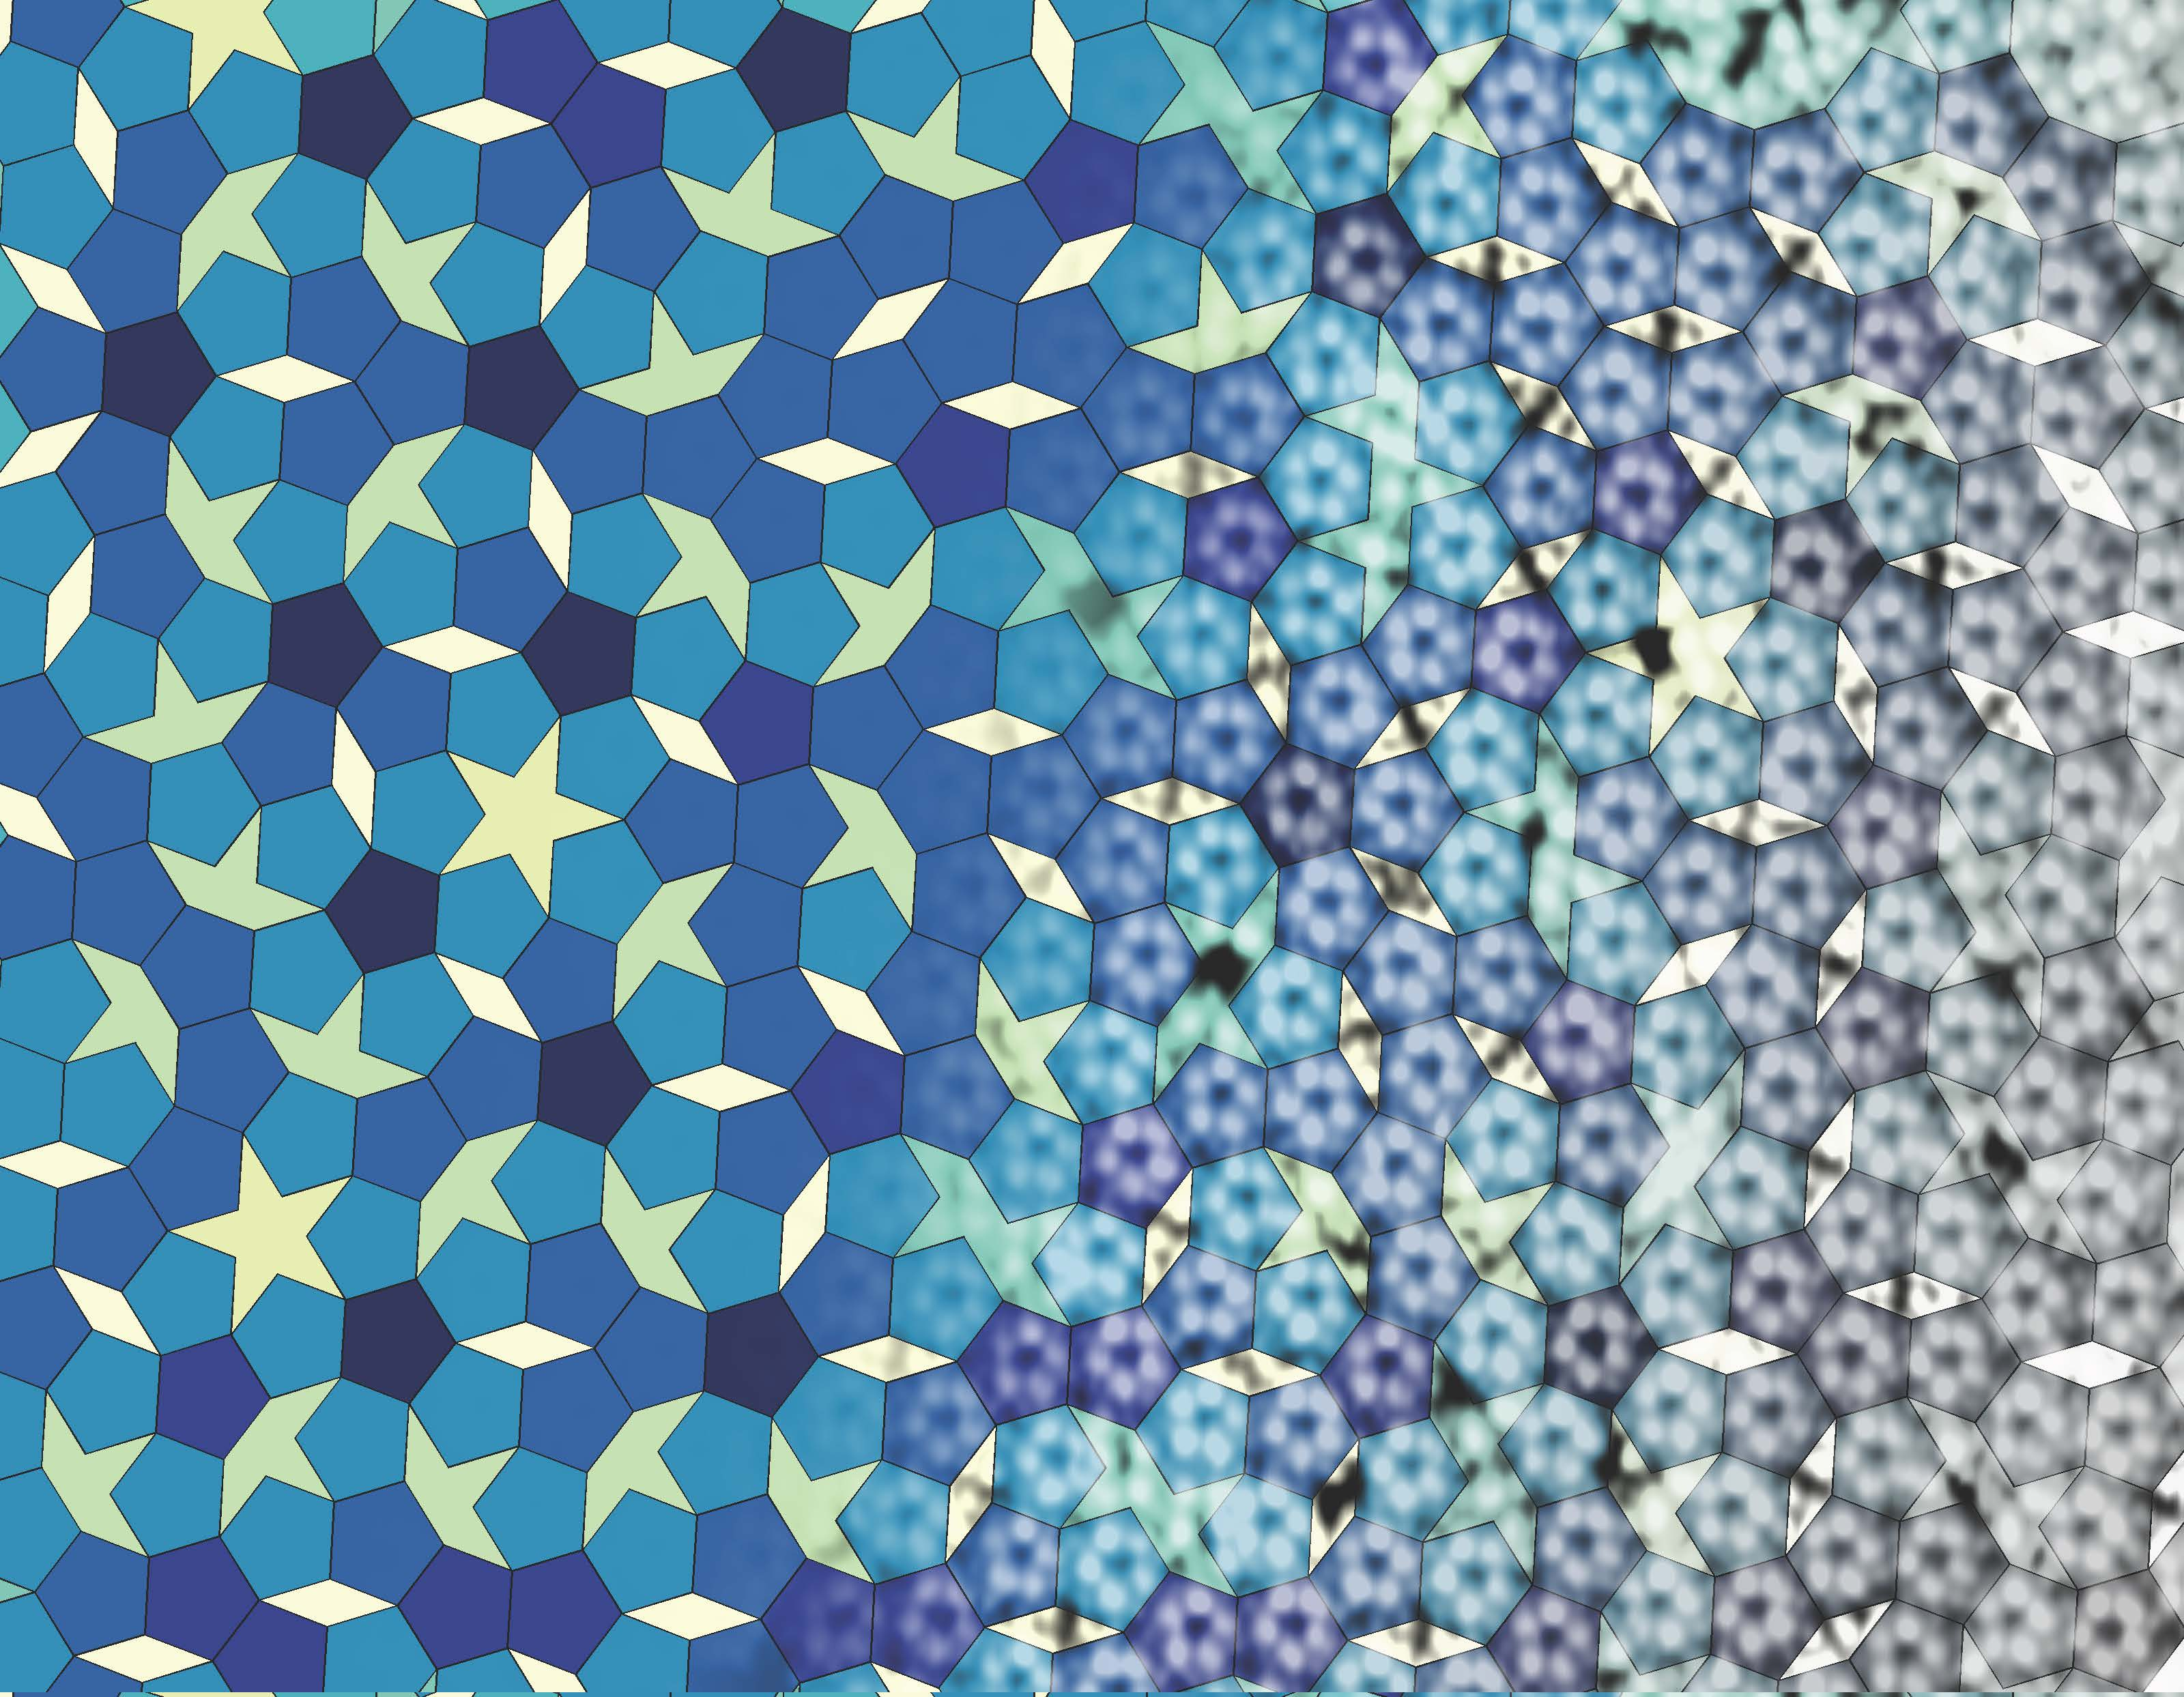
\includegraphics[scale=0.22]{img/1_intro/wasio.jpg}
		
		\ss{A 2D molecular quasicrystal} \ss{(\url{doi:10.1038/nature12993})}
	\>
\)

\begin{itemize}
	\item many intermetallic alloys are quasiperiodic
	\item a single natural example: Khatyrka meteorite hosts quasicrystals \ss{(\url{doi:10.1126/science.1170827})}. 
\end{itemize}
\end{frame}


\end{document}